\chapter{Opis wybranych algorytmów do przetwarzania chmur punktów w systemach GIS}

\section{Pozyskiwanie danych LiDAR}
LiDAR (z ang. \textit{Light Detection and Ranging}) jest nowoczesną metodą pozyskiwania informacji dotyczących wysokości terenu \cite{Marmol2003}.
Efektem jej działania jest tzw “chmura punktów”, która uwzględnia wysokość nie tylko powierzchni ziemi, ale również drzew, budynków itp.

Dane zbierane są za pomocą aparatury umieszczonej w samolotach (helikopterach), na którą składają się odbiornik GPS służący do określania
pozycji, czujnik INS pozwalający na określenie aktualnego przechyłu pojazdu oraz laser
LRF mierzący odległość \cite{WBPW2012}. Wykorzystuje on zakres podczerwieni (najczęściej fale o długości 1064nm) lub rzadziej fale z zakresu
światła widzialnego. Laser ten działa impulsowo, z częstotliwoścami rzędu kilkudziesięciu lub nawet kilkuset kHz, co w praktyce oznacza
próbkowanie nawet kilkuset tysięcy punktów na sekunde. Typowo promień lasera skierowany jest poprzecznie do kierunku lotu. W wyniku ruchu samolotu
uzyskuje się podczas jednego przelotu dane z pewnego, stosunkowo wąskiego, paska terenu, co schematycznie przedstawiono na rysunku \ref{fig:lidar}.

\begin{figure}[h!]
\centering
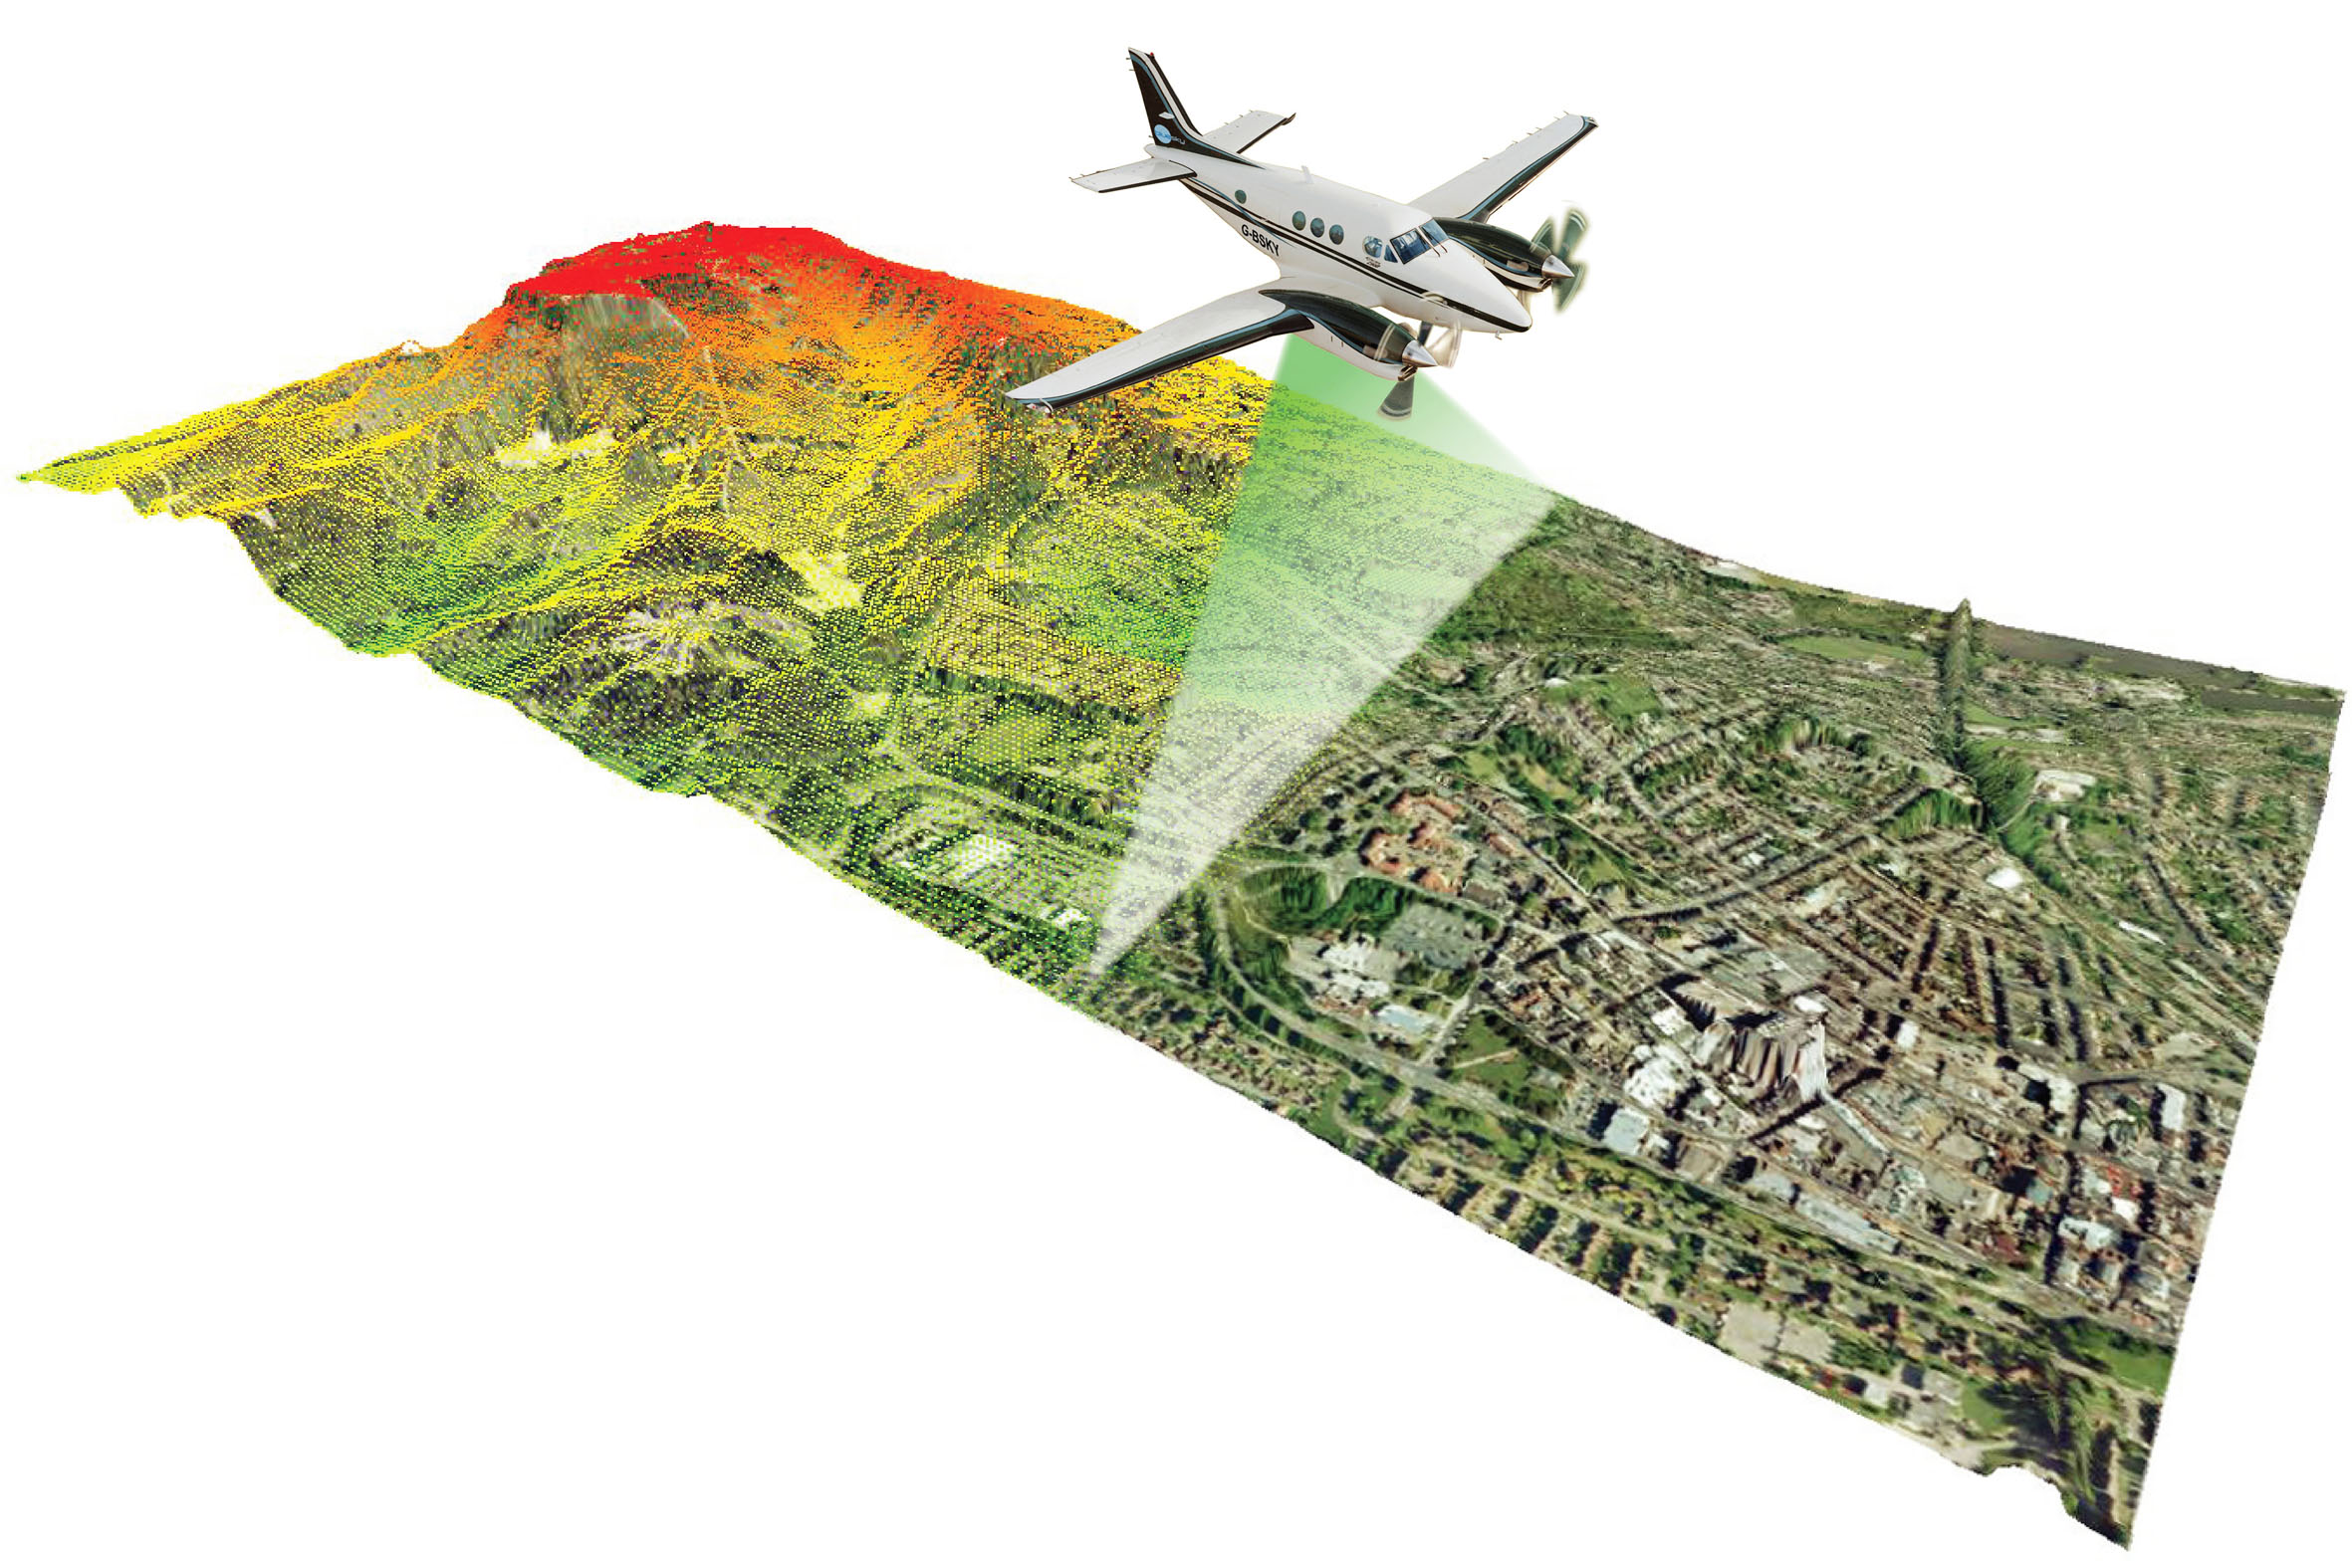
\includegraphics[width=0.9\textwidth]{img/LIDAR.jpg}
\caption{Schematycznie przedstawiony nalot podczas zbierania danych LIDAR}
\label{fig:lidar}
    \source{http://antyweb.pl/wp-content/uploads/2015/03/LiDAR-Escaneo-Ejemplo.jpg}
\end{figure}

Część wiązki odbija się od powierzchni i wraca do odbiornika. Na podstawie czasu odbicia określana jest odległość. Jako że odległości między
lecącym samolotem a powierzcnią ziemi są dosyć znaczne, konieczne jest wykorzystanie skanera o większej mocy, niż w typowych dalmierzach laserowych.
Z każdym odczytem powiązane są informacje z systemów GPS oraz INS. Pozwalają one na mierzenie (z wysoką częstotliwością) położenia oraz wychylenia samolotu.
W rezultacie umożliwia to perfekcyjne umieszczenie mierzonego punktu w przestrzeni.

Możliwe jest także rejestrowanie kilku odbić (tzw. ech) dla pojedynczego impulsu laserowego. W sytuacji, gdy impuls trafi na obszar zadrzewiony dojdzie do częściowego odbicia
od korony drzewa, zaś reszta energi przejdzie przez koronę i dobije się od gruntu. Ponadto, pomiędzy tymi skrajnymi odbiciami mogą wystąpić odbicia pośrednie.
Istnieją różne systemy rejestrujące odbitą falę, w tym:
\begin{itemize}
    \item Rejestrujące tylko pierwsze lub ostatnie odbicie,
    \item Rejestrujące pierwsze i ostatnie odbicie,
    \item Rejestrujące do pięciu odbić,
    \item Rejestrujące pełny kształ fali powracającej.
\end{itemize}

Ilość rejestrowanych odbić ma kluczowe znaczenie dla stosowania systemu. Za pomocą rejestrowania dwóch bądź więcej odbić możliwe jest określenie np:
wysokości drzew. Należy zaznaczyć, iż dla impulsów, które natrafią na powierzchnię gruntu, dachy budynków itp. zarejestrowane zostanie tylko jedno
odbicie.

Wielokrotność odbić wynika z faktu, iż promień laserowy ma w istoście pewną rozbierzność w wyniku której ślad lasera w terenie ma kształ elipsy.
Jej rozmiar jest zależny od kąta zbieżności promienia, wysokości lotu oraz kąta, pod którym promień trafia na ziemię. Ponadto dodaktowy wpływ ma
też nachylenie terenu. W związku z powyższym, jeżeli rozbierzna wiązka przechodzi częsciowo przez koronę drzew, następują wielokrotne odbicia części wiązki,
co pokazano na rysunku \ref{fig:lidar_beam}.

\begin{figure}[h!]
    \centering
    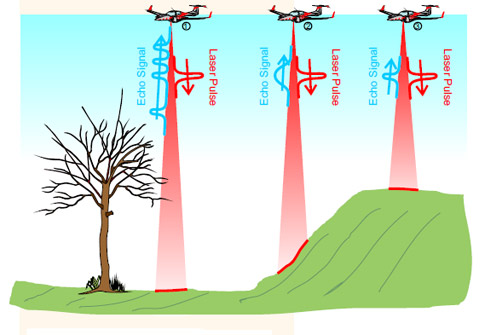
\includegraphics[width=0.9\textwidth]{img/lidar_beam.jpg}
    \caption{Kształt sygnału laserowego powracającego w zależności od typu powierzchni}
    \label{fig:lidar_beam}
    \source{http://www.qualitydigest.com/IQedit/Images/MISC\%20News\%20Pics/October\%2010/riegel-fig1.jpg}
\end{figure}

Na rysunku \ref{fig:lidar_beam} widać jak przedstawia się sygnał powracający do odbiornika. W przypadku przechodzenia przez koronę drzewa składa się on z kilku
maksimów, przy odbiciu od powierzchni gruntu - z jednego. Maksima te traktowane są jako punktowe odbicia od powierzchni o określonej odległości od samolotu i są traktowane
jako osobne echa.

Różne obiekty w różnym stopniu odbijają energię. Dla laserów działających w bliskiej podczerwieni najmniejsze odbicie występuje od powierzchni wody,
zaś największe od lodu i śniegu. Mała ilość odbitej energii może doprowadzać do powstawania tzw. "martwego pola" w skanowanym obszarze. Ponadto, niektóre
systemy skanują też intensywność sygnału powrotnego dając w efekcie obraz intensywności. Jest to źródło dodatkowych danych mogących służyć do dalszej analizy.

Martwe pola mogą powstawać także w innych sytuacjach. Jednym z nich jest skanowanie gęstego terenu zalesionego, w którym cała wiązka odbija się od koron drzew
nie docierając nigdy do powierzchni gruntu. Niweluje się ten efekt poprzez wykonywanie pomiarów w sezonie jesienno-zimowym (brak liści zwiększa prawdopodobieństwo
na dotarcie sygnału do powierzchni ziemi). Dodaktowo można zmniejszyć kąt, pod którym wiązka lasera pada na ziemię, co również ułatwia jej dotarcie do gruntu,
jak pokazano na rysunku \ref{fig:lidar_tree}. Martwe pole może też powstać poprzez zasłonięcie pewnej powierzchni przez wysokie budynki. W celu ich wyeliminowania
staosuje się wiele nalotów nad tym samym terenem, jednakże z różnych kierunków. Dane pochodzące z każdego nalotu są następnie łączone w jedna chmurę punktów \cite{isok_manual}.

\begin{figure}[h!]
    \centering
    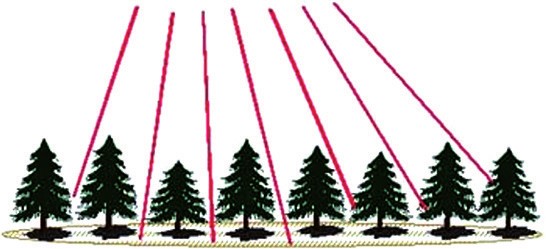
\includegraphics[width=0.9\textwidth]{img/lidar_tree.png}
    \caption{Penetracja impulsów laserowych jest zależna od kąta padania}
    \label{fig:lidar_tree}
    \source{http://www.gugik.gov.pl/\_\_data/assets/pdf\_file/0019/23752/PODRECZNIK\_ISOK\_wyd.2.pdf}
\end{figure}


\section{Triangulacja Delaunay'a}

Triangulacja Delaunay'a jest reprezentacją chmury punktów w postaci nieregularnej siatki trójkątów TIN (z ang. Triangulated Irregular Network).
Jej cechą szczególną jest fakt, iż żaden z punktów nie leży wewnątrz okręgu opisanego na dowolnym trójkącie \cite{Lee1980}. Podział ten ma tę własność, że maksymalizuje najmniejszy kąt spośród 
wszystkich trójkątów należących do triangulacji. Na rysunku \ref{fig:triangulacja} przedstawiono przykładową triangulacje.

\begin{figure}[h!]
    \centering
    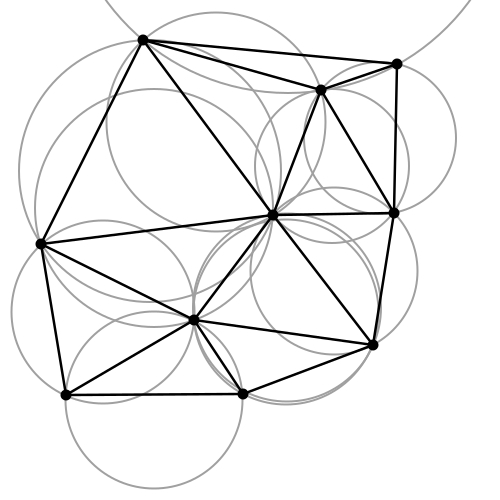
\includegraphics[width=0.3\textwidth]{img/triangulacja.jpg}
    \caption{Triangulacja Delaunay z zaznaczonymi okręgami opisanymi na trójkątach}
    \label{fig:triangulacja}
\end{figure}

Triangulacja Delaunay'a jest często wykorzystywana przy przetwarzaniu danych LIDAR. Dzięki stosowaniu filtracji może służyć do oddzielania poszczególnych zbiorów punktów od siebie \cite{koziol2007} bądź też do znajdywania łamanej otaczającej zadany zbiór punktów \cite{website:HumanGeoBlog}. Istnieje wiele implementacji algorytmu pozwalającego na przetworzenie chmury punktów do postaci siatki trójkątów \cite{Lee1980,Dwyer1987,jiang2010}. W artykule \cite{Lee1980} opisano dwa algorytmy tworzenia takiej siatki - dziel i zwyciężaj oraz tribuild. Pierwszy z nich o złożoności obliczeniowej $O(N log N)$ rekurencyjnie dzieli zbiór punktów pośrednich na mniejsze zbiory, w nich dokonuje triangulacji a następnie łączy je. Drugi z nich o złożoności obliczeniowej $O(N^{3/2})$ zakłada znajomość prostokąta który otacza zadany zbiór punktów. Prostokąt ten jest dzielony na mniejsze, a następnie dla każdego mniejszego prostokąta:
\begin{algorithmic}
    \For {punkt P w punktach należących do prostokąta}
    \If {P jedyny punkt w prostokącie}
        \State połącz punkt z wierzchołkami prostokąta
    \Else
        \State dodaj krawędzie, aby nie zniszczyć triangulacji
    \EndIf
    \EndFor
\end{algorithmic}

Przykładowe kolejne etapy tak przeprowadzonej triangulacji pokazano na rysunku \ref{fig:iter_triangulacja}.

\begin{figure}[h!]
    \centering
    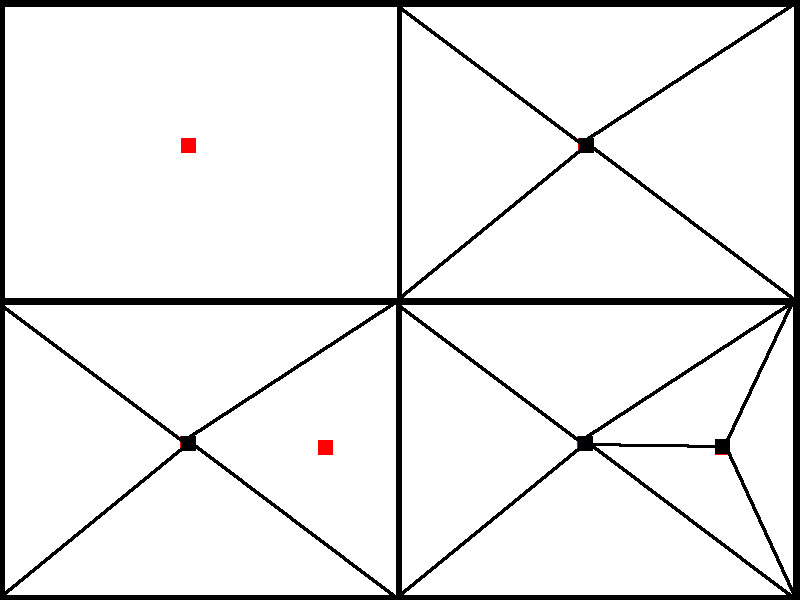
\includegraphics[width=0.4\textwidth]{img/iter_triangulacja.jpg}
    \caption{Iteracyjna triangulacja}
    \label{fig:iter_triangulacja}
\end{figure}

W 1987 Dwayer zaproponował szybszy algorytm dziel i zwyciężaj, o zakładanej złożoności $O(N log log N)$, jednak w pesymistycznym przypadku dalej będzie
to $O(N log N)$  \cite{Dwyer1987}. Powstały też nowsze algorytmy pozwalające na stworzenie triangulacji.
W \cite{jiang2010} autorzy zwracają uwagę, że w większości algorytmów szybko tworzy się siatkę a następnie dużo czasu poświęca się na lokalne optymalizacje,
co skutkuje zwiększoną złożonością obliczeniową. Dzięki zaproponowaniu reguły prawej dłoni, udało im się znacząco zmniejszyć
ilość obliczeń potrzebnych do przeprowadzenia lokalnych optymalizacji, tym samym proponowany algorytm ma złożoność na poziomie $O(N)$.

\section{Maszyny wektorów nośnych}

Maszyny wektorów nośnych SVN (z ang. \textit{support vector machine}) pozwalają na rozwiązanie tzw. problemu klasyfikacji. Definicja problemu brzmi następująco: dla pewnej przestrzeni $\Omega$ zawierającej wektory danych x, należące do dwóch klas
$\Omega = \{(x_{i}, c_{i}) | x_{i} \in R^p, c_{i} \in \{-1,1\}\}$
(gdzie $p$ oznacza ilośc wymiarów wektora $x$) należy znaleźć klasyfikator który podzieli tę przestrzeń na dwa rozłączne obszary jak najlepiej
odpowiadające klasom $\{-1, 1\}$ \cite{stefanowski2010}. Do rozdzielenia zbioru na dwa służy tzw. liniowa funkcja separująca
(lub jej uogólnienie - hiperpłaszczyzna dla przypadków n-wymiarowych), która wyznacza podział przestrzeni na dwa podobszary.

\begin{figure}[h!]
    \begin{subfigure}[b]{0.33\textwidth}
        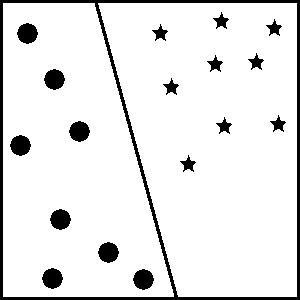
\includegraphics[width=\linewidth]{img/granica_1.jpg}
    \end{subfigure}%
    \begin{subfigure}[b]{0.33\textwidth}
        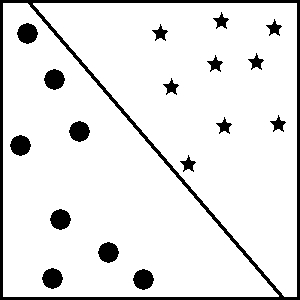
\includegraphics[width=\linewidth]{img/granica_2.jpg}
    \end{subfigure}%
    \begin{subfigure}[b]{0.33\textwidth}
        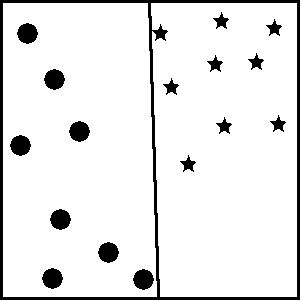
\includegraphics[width=\linewidth]{img/granica_3.jpg}
    \end{subfigure}
    \caption{Różne przykłady liniowej separacji}
    \label{fig:liniowa_separacja}
\end{figure}

Na rysunku \ref{fig:liniowa_separacja} przedstawiono różne poprawne sposoby separowania tego samego zbioru. Można w szczególności wyróżnić pary hiperpłaszczyzn $b_{i1}$ oraz $b_{i2}$, będących równoległych do 
siebie, powstałych poprzez przesuwanie jednej hiperpłaszczyzny od punktu granicznego pierwszego zbioru do punktu granicznego drugiego zbioru (rysunek \ref{fig:rownolegla_separacja}).
\newpage
\begin{figure}[h!]
    \centering
    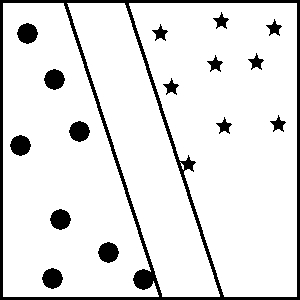
\includegraphics[width=0.33\textwidth]{img/granica_rownolegla.jpg}
    \caption{Równoległe hiperpłaszczyzny dla przypadku dwuwymiarowego}
    \label{fig:rownolegla_separacja}
\end{figure}

Odległości pomiędzy hiperpłaszczyznami $b_{i1}$ oraz $b_{i2}$ nazywamy marginesem klasyfikatora liniowego. Maszyny wektorów nośnych znajdują taką hiperpłaszczyznę, która maksymalizuje margines. Szukamy więc hiperpłaszczyzny spełniającej warunki:

\begin{equation}
    w*x + b =0
\end{equation}

gdzie $w$ i $b$ są parametrami modelu. Wtedy przynależność do klas można wyrazić jako:

\begin{displaymath}
    y = \left\{ \begin{array}{ll}
        1 & \textrm{$w*x+b>0$}\\
        -1 & \textrm{$w*x+b<0$}\\
    \end{array} \right.
\end{displaymath}

Parametry $w$ i $b$ należy wyznaczać tak, aby maksymalne marginesy $b_{i1}$ i $b_{i2}$ były miejscem geometrycznym punktów $x$ spełniających warunki:
\begin{eqnarray}
    b_{i1} \quad w*x + b =1 \\
    b_{i2} \quad w*x + b =-1
\end{eqnarray}

Możliowości wykorzystania maszyn wektorów nośnych do przetwarzania chmury punktów nasuwają się same - możliwe jest chociażby przydzielanie punktów do klas drzew i budynków \cite{xwang2011}. Istnieje wiele 
różnych przykładów na wykorzystanie SVN do przetwarzania chmur punktów \cite{xwang2011,li2013,david2015}. We wszystkich z nich część punktów pomiarowych jest wykorzystywana jako dane uczące.
Dla tych punktów operator ręcznie przydziela je do jednej z klas \cite{xwang2011}. Następnie na podstawie tych punktów możliwe jest określenie najlepszej hiperpłaszczyzny, jak opisano w sekcji \textit{definicja}.
W \cite{xwang2011} wykorzystano tzw. niezbalansowane maszyny wektorów nośnych USVN (z ang. \textit{unbalanced support vector machines}) do rozróżnienia drzew i budynków.
Do analiz autorzy wykorzystali zdjęcia satelitarne oraz dane pochodzące z LIDARa - za pomocą tych dwóch źródeł stworzono wektory $x$
składające się z wysokości $Z$, wariancji wysokości $sZ$, różnice wysokości $hZ$,
pochodne 3-go rzędu wzdłuż osi X i Y - odpowiedno $dX$ i $dY$ - oraz wartość koloru RGB ze zdjęcia satelitarnego. 
W \cite{li2013} wykorzystano SVM do przypisywania punktów do więcej niż dwóch klas. 
W \cite{david2015} równierz wykorzystano SVM do podziału zbioru na więcej niż dwie klasy. Analiza to posłużyła do zmierzenia powierzchni namorzyn na Filipinach. 
W tym przypadku do stworzenia wektorów $x$ wykorzystano numeryczny model powierzchmi DSM, numeryczny model terenu DTM, model wysokościowy CHM, średnią intensywność oraz ilość odbić. Co ciekawe, na podstawie
ilości odbić można określić gatunek drzewa \cite{Sasaki2012}.

\section{Analiza OBIA}

Analiza obrazu oparta obiektowo OBIA (z ang. \textit{Object – based image analysis}) jest stosunkowo nową metodą \cite{burnett2003} służącą do przetwarzania obrazów. W przeciwieństwie do tradycyjnych metod przetwarzania, 
nie analizuje pojedynczych pikseli, lecz całe ich grupy, zwane obiektami. Ma to przypominać sposób, w jaki ludzie rozróżniają obiekty na zdjęciach. Jeżeli zdjęcia dotczą powierzchni ziemi (takie jak zdjęcia 
satelitarne) wyróżnia się wtedy metodę geograficznej analizy obrazu oparte obiektowo GEOBIA (z ang. \textit{Geographic Object-based Image Analysis}). Jako że tematyka całej pracy dotyczy systemów GIS,
w dalszej części będzie opisywana ten szczególny przypadek OBIA.

Metoda ta składa się z dwóch etapów. w Pierwszym z nich grupuje się podobne piksele (np. pod względem koloru) w obiekty prymitwne (prymitywy). Prymitywy służą następnie do konstruowania bardziej złożonych 
struktur, odpowiadających rzeczywistym obiektom takim jak jeziora czy drogi \cite{Blaschke2014}.  Budowanie obiektów może odbywać się stopniowo na poziome wielu wartstw, jak przedstawiono na rysunku
\ref{fig:poziomy_struktury}.

\begin{figure}[h!]
    \centering
    \includegraphics[width=0.5\textwidth]{img/obiekowa_analiza.png}
    \caption{Podział obrazu na piksele i obiekty}
    \label{fig:poziomy_struktury}
\end{figure}

Metoda ta jest szeroko używana do analizy danych pochodzących ze skanowania laserowego. Jest wykorzystywana do klasyfikowania terenów miejskich \cite{zhou2013,chen2014},
wykrywania zmian powierzchni lasu \cite{zhang2014} oraz do wspomagania zarządzania terminalem kontenerowym \cite{tiede2015}. W tym ostatnim wykorzystano technikę OBIA do dokładnego określania miejsca położenia
kontenerów. Jest to zadanie o tyle łatwiejsze, iż wielkość kontenerów jest znana i podana jako norma ISO 668. Do celów analizy stworzono model DTM na podstawie danych LIDAR. Następnie do wykrywania
umiejscowie kontenerów wykorzystano dane LIDAR (pochodzące z jednego nalotu) oraz wykonywane częściej zdjęcia. Efektem jest model 3D nabrzeża.

Na polu analizy i klasyfikacji terenów miejskich metoda OBIA również odnosi sukcesy. Jednym z przykładów jest praca opisana w artkule z 2014 roku \cite{chen2014} w której autorzy za pomocą jedynie
danych LIDAR uzyskali dokładność klasfikacji punktów na poziomie  96.3\%. Wykorzystano w tym celu cztery informacje pochodzące ze skanowania - wysokość punktów nad poziomem gruntu, intensywność (czasem
nazywana amplitudą) oraz różnicę wysokości i intensywności pierwszego i ostatniego impulsu. Następnie podzielono obraz na prymitywy, jak opisano w sekcji Definicja. Na końcu nastąpiło przypisanie poszczególnych
obiektów do różnych klas na podstawie opisanych powyżej czterech atrybutów, jak przedstawia tabelka \ref{tab:przypisanie_do_klas}.

\begin{table}[h!]
    \centering
    \caption{Klasyfikacja terenów na podstawie cech}
    \label{tab:przypisanie_do_klas}
    \begin{tabular}{|c|c|c|c|}
        \hline
        Klasa & Wysokość & Intensywność & Różnica wysokości i intensywności\\
        \hline
        Trawniki & Niska & Wysoka & Bardzko niska\\
        \hline
        Trawa i roślinność & Niska & Średnia & Bardzo niska\\
        \hline
        Drogi i ziemia & Niska & Niska & Bardzo niska\\
        \hline
        Woda & Niska & Bliska 0 & Bardzo niska\\
        \hline
        Krzewy & Średnia & Średnia & Niska\\
        \hline
        Infrastruktura Publiczna & Średnia & Wysoka & Średnia\\
        \hline
        Drzewa & Duża & Wysoka & Duża\\
        \hline
        Budynki & Duża & Wysoka & Średnia\\
        \hline
    \end{tabular}
\end{table}

\section{Analiza Głównych Składowych}

Analiza głównych składowych (z ang. \textit{Principal component analysis PCA}) to metoda statystyczna służąca do analiz wielowymiarowych, polegająca na tworzeniu nowych zmiennych nazywanych głównymi składowymi.
Są one tworzone w taki sposób, aby kilka pierwszych z nich opisywało w dużym stopniu zmienność modelu (miały jak największą wariancję). Algebraicznie, główne składowe są szczególnymi kombinacjami liniowymi $p$
zmiennych losowych $X_{1}, X_{2}, \cdots, X_{p}$. Geometrycznie jest to przesunięcie układu współrzędnych. Po tranformacji osie układu reprezentują kierunki
z maksymalną wariancją\cite{johnson2002}.

Niech dla wektora zmiennych losowych $X'=[X_{1}, X_{2}, \cdots, X_{p}]$, posiadającego macierz kowariancji $\Sigma$ z wartościami własnymi $\lambda_{1} \geqslant \lambda_{2} \geqslant ... \geqslant \lambda_{p}
\geqslant 0$. Rozważmy wtedy kombinacje liniowe:
\begin{align}
    \begin{split}
        Y_{1} &= a'_{1}X = a_{11}X_{1} + a_{12}X_{2} + \cdots + a_{1p}X_{p} \\
        Y_{2} &= a'_{2}X = a_{21}X_{1} + a_{22}X_{2} + \cdots + a_{2p}X_{p} \\
        &\vdots \\
        Y_{p} &= a'_{p}X = a_{p1}X_{1} + a_{p2}X_{2} + \cdots + a_{pp}X_{p}
    \end{split}
\end{align}

Wtedy można wykazać że:
\begin{align}
    Var(Y_{i} = a'_{i}\Sigma a_{i} \quad i = 1,2, \cdots, p 
    \label{eq:wariancja} \\
    Cov(Y_{i}, Y_{k}) = a'_{i} \Sigma a_{k} \quad i,k = 1,2, \cdots, p
\end{align}

gdzie $Var$ i $Cov$ to odpowiednio wariancja i kowariancja. Główne składowe to te \textit{nieskorelowane} kombinacje liniowe $Y_{1}, Y_{2}, \cdots, Y_{p}$ których variancje w \ref{eq:wariancja} są
największe.

W przypadku analizy chmury punktów PCA wykorzystywana jest do wyznaczania własciwości lokalnej geometrii \cite{natale2010} czy do określania gatunków drzew \cite{lee2016}.
W tym pierwszym przypadku analizowano dane LIDAR pochodzące ze skanowania naziemnego w celu usunięcia szumów oraz wykrycia powierzchni brył (takich jak domy).
PCA było tylko częścią analizy, pomagającą określić czy zadany punkt jest pojedynczym punktem (traktowanym jako błąd, ergo przeznaczonym do usunięcia), fragmentem lini (tym samym najprawdopodobniej krawędzi)
czy też fragmentem powierzchni.
W drugiej z cytowanych prac autorzy postawili sobie za cel określenie jakiego gatunku są pojedyncze zdjęcia na podstawie zdjęć lotniczych i danych LIDAR.
Ze względu na mnogość danych, zdecydowali się na wykorzystanie PCA aby zmniejszyć ilość zmiennych a tym samym - przyspieszyć obliczenia.

\section{Ukryte Modele Markowa}

Ukryte modele markowa HMM (z ang. \textit{Hidden Markov Model}, czasem nazywane też łańcuchami Markowa) to metoda statystyczna służąca do modelowania procesów.
Na rysunku \ref{fig:lancuch_markova} przedstawiono przykładowy model.
Składa się on ze stanów (X, Y, Z), prawdopodobieństwa przejść między nimi oraz emisji które są stowarzyszone z każdym ze stanów.
Jeżeli zaobserowawliśmy sekwencję $2-1-1$, to wiemy że byliśmy kolejno w stanach $Y-X-X$ \cite{blunsom2004}. 

\begin{figure}[h!]
    \centering
    \includegraphics[width=1.0\textwidth]{img/HMM.png}
    \caption{Łańcuch Markowa}
    \label{fig:lancuch_markova}
\end{figure}

\newpage

Formalna definicja ukrytych modeli markowa prezentuje się następująco:
\begin{equation}
    \lambda = (A,B,\pi)
\end{equation}

$S$ jest zbiorem stanów, a $V$ zbiorem obserwacji:
\begin{align}
    S = (s_{1}, s_{2}, \cdots, s_{N}) \\
    V = (v_{1}, v_{2}, \cdots, v_{M}) 
\end{align}

Definiujemy $Q$ jako sekwencję przejść o stałej długości $T$ i powiązaną z nim sekwencję obserwacji $O$:
\begin{align}
    Q = q_{1}, q_{2}, \cdots, q_{T} \\
    O = o_{1}, o_{2}, \cdots, o_{T}
\end{align}

Macierz $A$ zawiera prawdopodobieństwa przejścia ze stanu $i$ do stanu $j$. Należy zaznaczyć, iż prawdopodobieństwa te są niezależne od czasu $t$:
\begin{equation}
    A = [a_{ij}], a_{ij} = P(q_{t} = s_{j} | q_{t-1} = s_{i})
\end{equation}

$B$ jest macierzą obserwacji. Zawiera prawdopodobieństwa zaobserwowania emisji $k$ przy staniej $i$, niezależnie od czasu $t$:
\begin{equation}
    B = [b_{i}(k)], b_{i}(k) = P (x_{t} = v_{k} | q_{t} = s_{i})
\end{equation}

$\pi$ jest macierzą określająca prawdopodobieństwa wystąpienia $i-tego$ stanu jako pierwszego:
\begin{equation}
    \pi = [\pi_{i}], \pi_{i} = P(q_{1} = s_{i})
\end{equation}

Dodatkowo poczyniono dwa założenia. Pierwszym z nich jest brak pamięci tzn. stan aktualny może zależeć tylko od stanu poprzedniego:
\begin{equation}
    P(q_{t}|q_{1}^{t-1}) = P(q_{t}|q_{t-1})
\end{equation}

Drugim założeniem jest niezależność, tzn. iż obserwacja z czasu $t$ jest zależna tylko od stanu z czasu $t$:
\begin{equation}
    P(o_{t}|o_{1}^{t-1},q_{1}^{t}) = P(o_{t}|q_{t})
\end{equation}

Ukryte modele markowa są najczęsciej wykorzystywane w zagadnieniach związanych z rozumieniem i syntezą mowy \cite{blunsom2004}, jednakże istnieją przykłady na wykorzystanie tej metody do przetwarzania
chmur punktów \cite{wang2014}. W pracy \cite{wang2014} wykorzystano HMM do stworzenia autonomicznego pojazdu. Metoda ta posłużyła do wykrywania typów powierzchni.

